\documentclass{article}
\usepackage{hyperref}
\usepackage{pdfpages}
\title{EMISY Project 21 Portable Compass}
\author{Krzysztof Rudnicki, 307585}
\date{\today}
\begin{document}
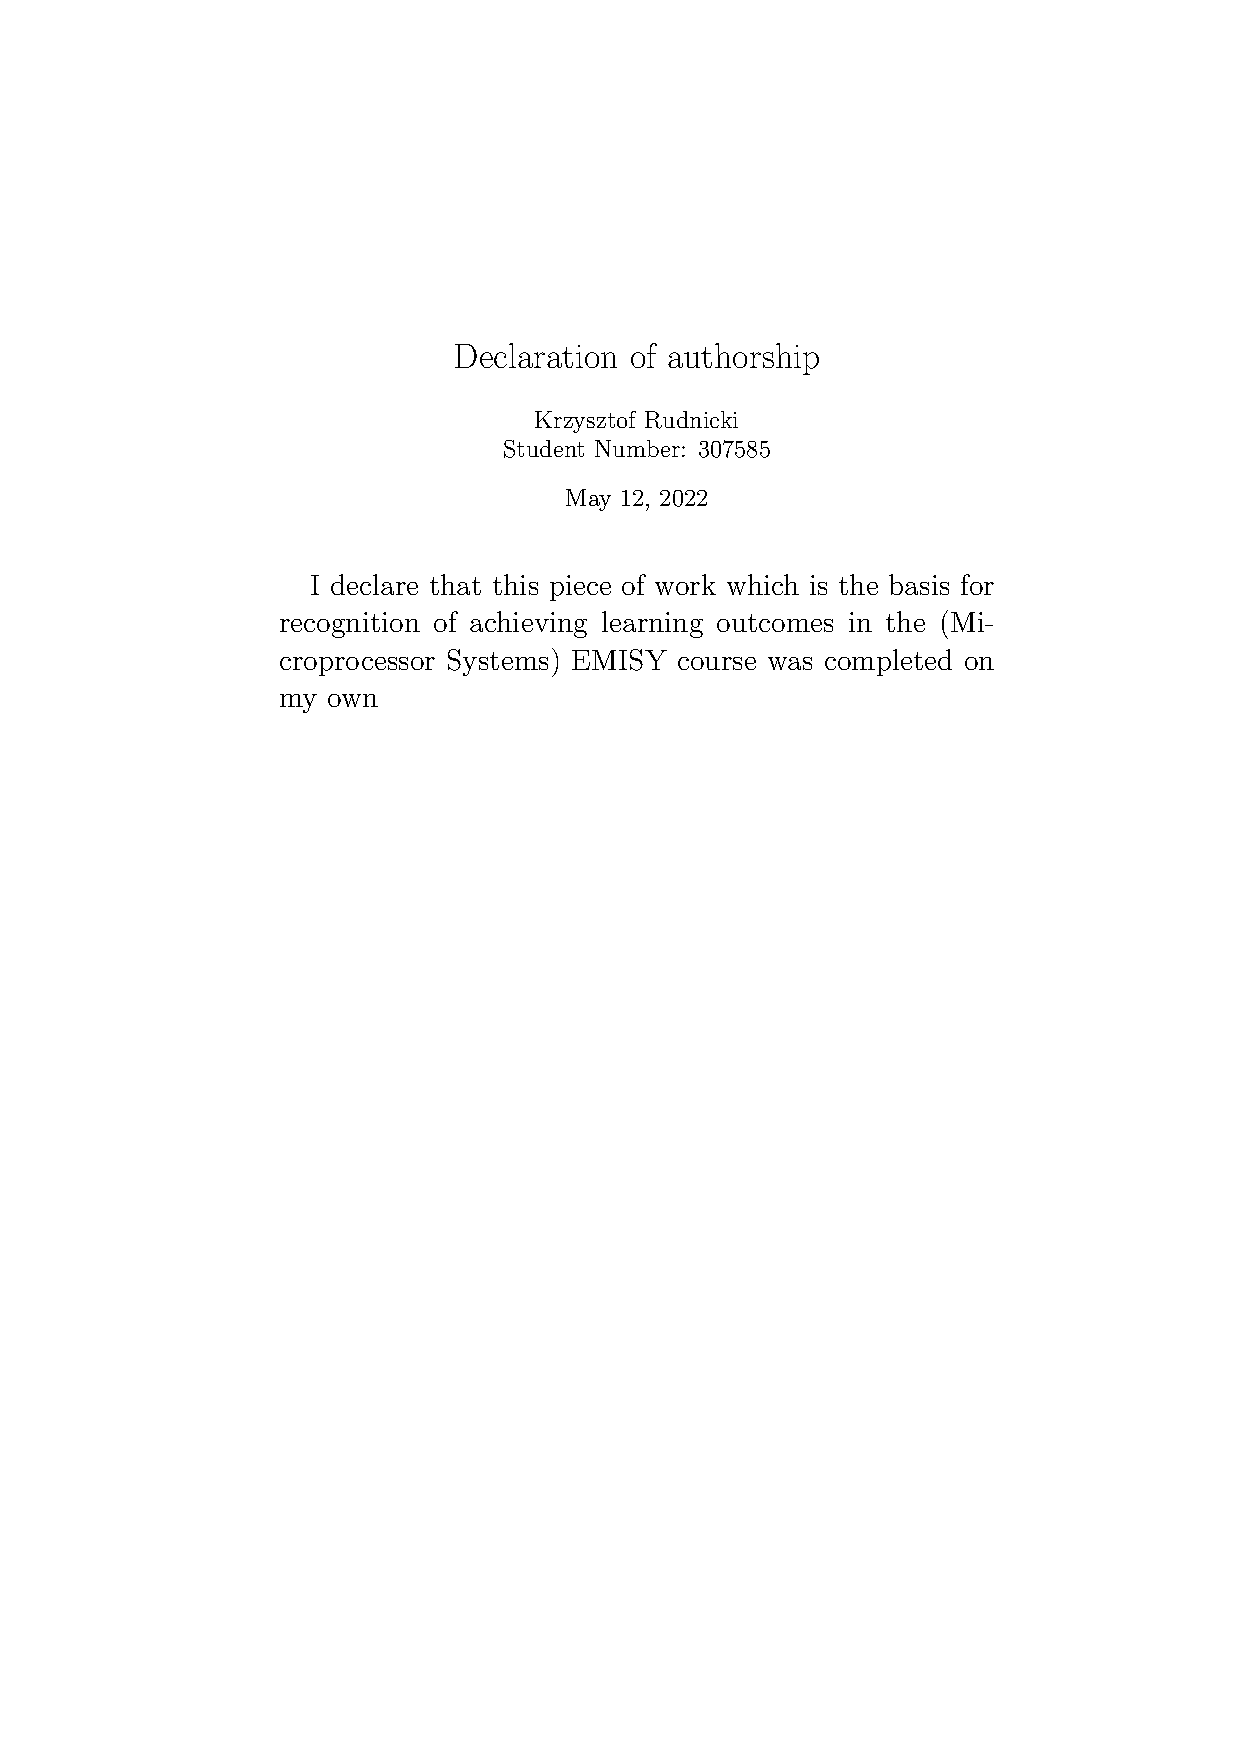
\includepdf[pages={1}]{declaration.pdf}
\maketitle
\section{Analysis of the project}
\subsection{Discussion of project requirements}
We need to create a simple portable compass circuit \\
It should:
\begin{itemize}
	\item Use energy-saving power modes of microcontroller
	\item Be battery powered
	\item Be portable (cellphone/wrist watch)
	\item Communicate using graphical OLED display and two buttons keyboard
\end{itemize}
\subsection{Discussion of solution}
In my solution I focused on picking components based on firstly low power
consumption, then size, then simplicity, whenever I could I tried to do
everything as proposed in the component data sheet. \\
For the schematic itself I needed power saving microcontroller, oled display,
battery, voltage regulator that works well with batteries and digital compass.
\section{Detailed circuit diagram}
\subsection{Diagram itself}
(Diagram is in pdf format so feel free to zoom in if something is not clearly
visible) 
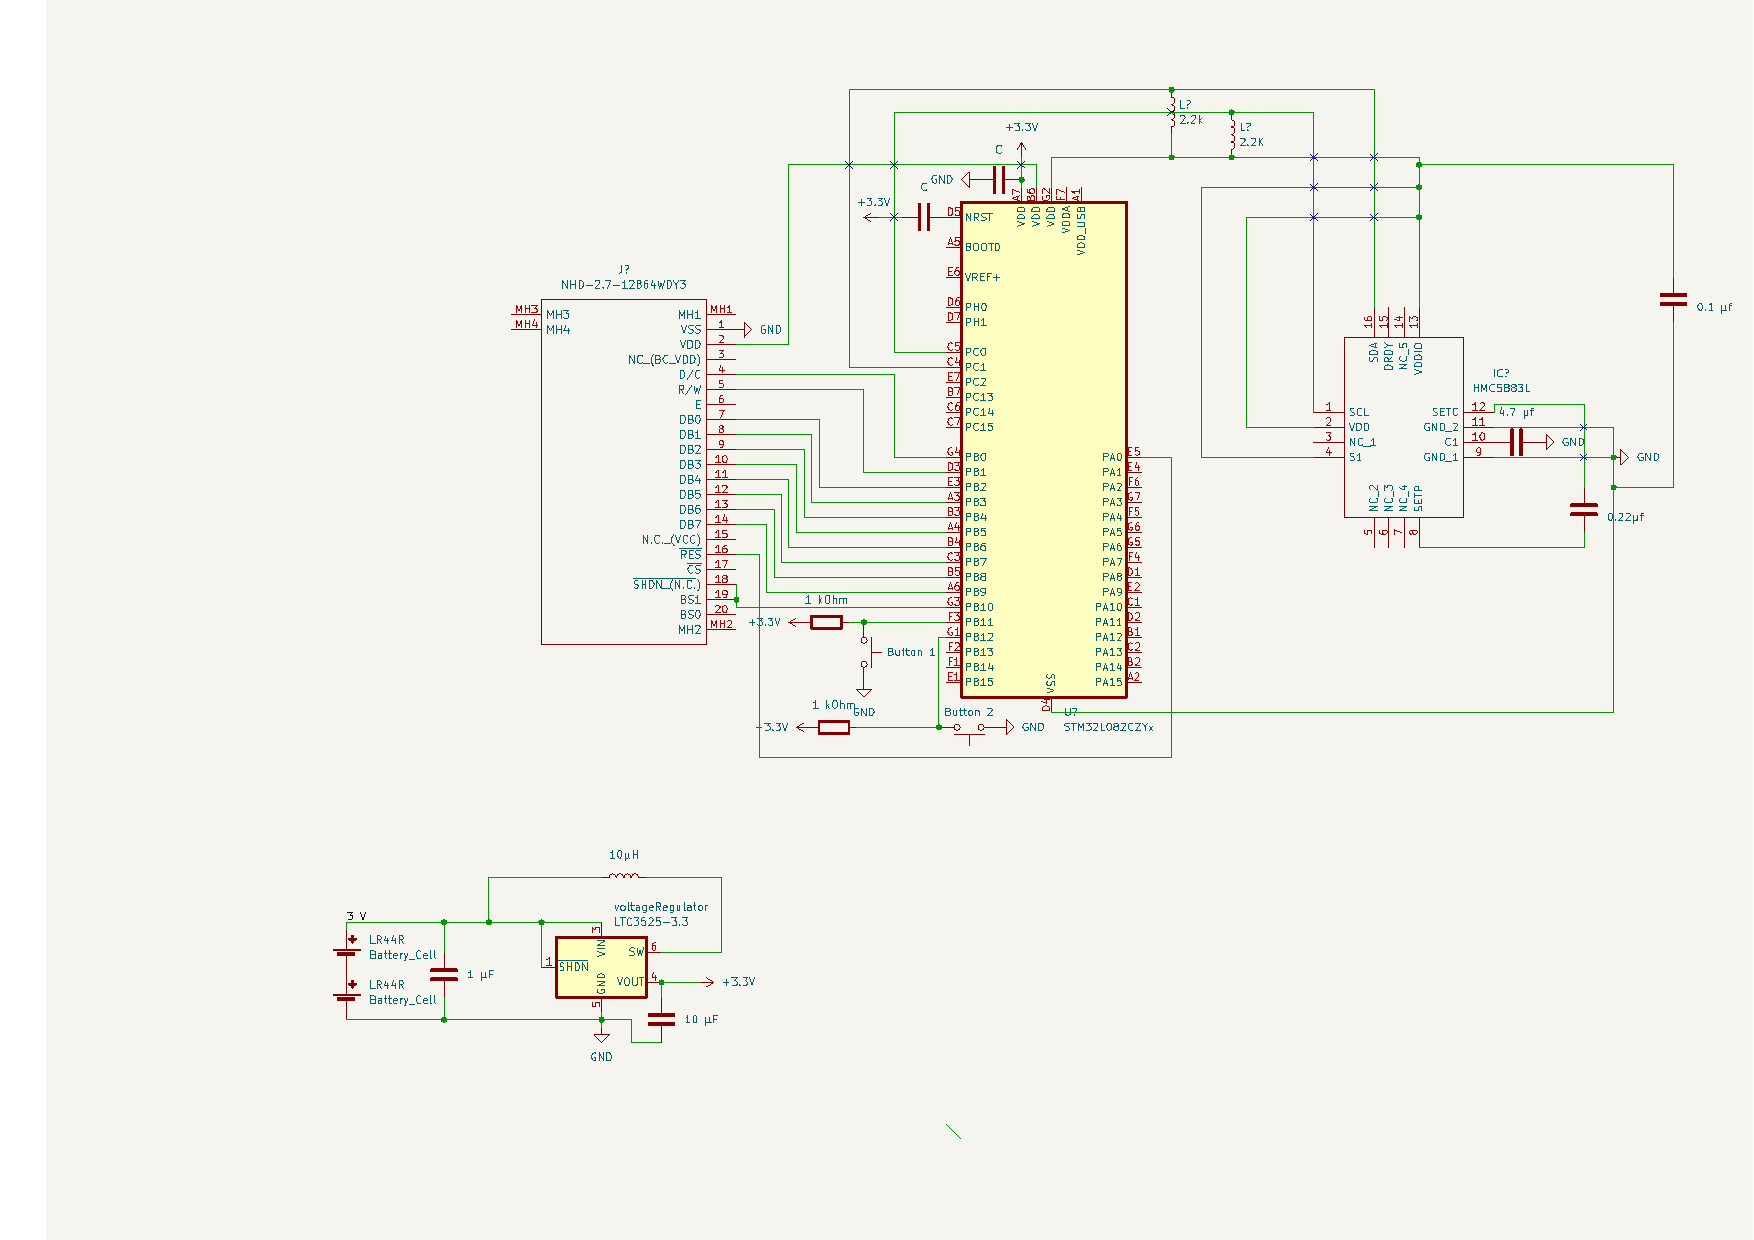
\includepdf[pages=-]{schematicpdf.pdf}
\subsection{Diagram description}
Voltage regulator schematic is done one to one on how it was done in voltage
regulator schematic in case of two battery cells \\ 
Digital compass also was connected exactly as specified in datasheet \\
For OLED I based on the pin descriptions from datasheet and on common patterns
of connecting peripherals \\
Microcontroller itself was pretty straightforward with classic VDD, VSS and
Reset pin conections \\
For buttons I used pull up resistors 
\newpage
\subsection{Components}
\subsubsection{Microcontroller}
I decided to use STM32L082CZ from STM32L0 line
\paragraph{Relatively small} Up to 10 mm $\times$ 10 mm dimensions, 
compared to apple watch display of 34 mm by 40 mm for smaller version. 
\cite{datasheet}
111th page
\paragraph{Square} It is shaped in a square which also simplifies portability
\cite{datasheet} 111th page
\paragraph{Power saving} STM32L0 line was designed specifically for low power
consumption with power consumption as low as 0.29 $\mu$ A in Standby mode
\cite{datasheet} 1st page
\paragraph{Consumer devices} This microcontroller comes from STM32LOx2 line
prepared to be used in consumer devices \cite{consumerDevice}
\paragraph{Ease of use} USB compatible microcontroller and dedicaded debug port
allows for swift code creation.
\cite{datasheet} 1st page 
\subsubsection{All other components}
\paragraph{Oled display} For OLED display I decided to go with
NHD-2.7-12864WDY3. It was an OLED display found on \href{www.mouser.pl}{mouser}
webpage with lowest operating supply current of 180 uA, supply voltage
compatible wit microcontroller (3.3 V) and datasheet not in japanese.
\cite{OLED}
\paragraph{Digital compass} For the compass I used HMC5883L with compatible
voltage, low power consumption of 100 $\mu$ A, compatiblity with battery powered
applications according to datasheet and small size 
\paragraph{Battery} For the battery I choose 2x LR44R series battery, with output
voltage of 1.5 V compatible with voltage regulator (3 V in series), compatible
battery chemistry of Alkaline, 150 mAh capacity for single battery and compact
coin cell shape. \cite{Battery}
\paragraph{Voltage Regulator} For voltage regulator I choose LTC3525-3.3 with high 95 \%
efficiency, desirable output voltage of 3.3 V, low profile and tiny package, it
is also available in kicad by default \cite{Voltage Regulator}
\section{Draft of the microcontroller firmware}
\subsection{Block diagram}
\subsection{Description of the algorithm}
\begin{thebibliography}{9}
	\bibitem{datasheet} 
	\href{https://www.st.com/resource/en/datasheet/stm32l082cz.pdf}{STM32LO82CZ
	datasheet}
	\bibitem{consumerDevice}
	\href{https://www.st.com/en/microcontrollers-microprocessors/stm32l0-series.html}{Consumer
	Device STM32LOx2 Line}
	\bibitem{OLED}
	\href{https://www.mouser.pl/datasheet/2/291/NHD_2_7_12864WDY3-1116258.pdf}{OLED
	datasheet}
	\bibitem{Magnetometer}
	\href{https://cdn-shop.adafruit.com/datasheets/HMC5883L_3-Axis_Digital_Compass_IC.pdf}{Magnetometer
	datasheet}
	\bibitem{Battery}
	\href{https://www.murata.com/products/productdata/8809693839390/LR44R-DATASHEET.pdf?1604287808000}{Battery}
	\bibitem{Voltage Regulator}
	\href{https://www.analog.com/media/en/technical-documentation/data-sheets/3525fc.pdf}{Voltage
	regulator} 
\end{thebibliography}
\end{document}

